\documentclass[journal, a4paper]{IEEEtran}
\usepackage{graphicx}
\usepackage{url}
\usepackage{subfigure}
\usepackage{float}
\usepackage{blindtext}
\usepackage{enumitem}
\usepackage{amsmath}
\usepackage{algorithm}
\usepackage[noend]{algpseudocode}
\usepackage{xspace}
\begin{document}

% Define document title and author
	\title{Trivial File Transfer Protocol}
	\author{Mateos Hoyos, Alfonso José \\ Luis Lazo, Gabino}
	\markboth{Práctica Sockets 2018 - TFTP}{}
	\maketitle

% Write abstract here
\begin{abstract}
	En esta práctica se documenta la realización del protocolo de transferencia de archivos TFTP, el cual está pensado para UDP, pero por motivos académicos también se ha implementado en TCP. En los posteriores puntos se comentan las diferencias en ambas implementaciones, además de las pruebas realizadas.
\end{abstract}

% Each section begins with a \section{title} command
\section{Introducción}
	En esta práctica se ha implementado el protocolo de transferencia de archivos TFTP, el cual es una versión más simple del protocolo FTP. La implementación consta de dos versiones, una para TCP y otra para UDP. Es importante tener en cuenta las principales diferencias de la aplicación dependiendo del protocolo de transporte:
\begin{itemize}
\item Para TCP es necesario tener en cuenta, ya que es un protocolo con conexión y asentimiento, que no son necesarios los ACK de cada paquete; no obstante, con la intención de seguir el protocolo, se han implementado los paquetes de asentimiento de bloques y mensajes de error.
\item Para UDP, ha sido necesario implementar timeouts en las funciones bloqueantes de recepcion de mensajes del socket, debido a que no existe conexión entre los participantes.
\end{itemize}	

Para asegurar la existencia de concurrencia en ambas implementaciones, cada conexión nueva se procesa en hilos diferentes.

En la siguientes secciones se detallan la arquitectura y las pruebas de funcionamiento realizadas.

% Main Part
\section{Arquitectura}
	El programa consta de 4 fuentes principales:
	\begin{itemize}
	\item packet.c: en este fuente se especifican las estructuras que se usan para el envío, recepción y procesamiento de los mensajes del protocolo. En concreto: 
	\begin{itemize}
	\item Estructura request\_msg: donde se guardan las cadenas filename y mode usadas en los mensajes de peticion de escritura o lectura. 
	\item Estructura data\_msg: la estructura principal de la aplicación para la transferencia de archivos, donde se guardan el número de bloque, el dato en concreto y el tamaño del mismo. 
	\item Estructura ack\_msg: que contiene el numero del bloque al cual se asiente. 
	\item Estructura err\_msg: donde se guarda un codigo y un mensaje de error. 
	\item Estructura packet: en la cual se guardan los mensajes típicos del protocolo para el procesamiento en la aplicación. El primer campo es el código de operación (2 bytes) y el segundo campo es una unión que contiene las estructuras anteriores.
	\end{itemize}
	Además, se implementan las funciones de serialización de la estructura packet para la transferencia del protocolo TFTP. 	
	\item transfer.c: en este fuente se encapsulan las funciones de transferencia de sockets, las cuales son diferente para UDP y TCP, utilizando dinámicamente ambos protocolos de transporte e implementando los timeouts correspondientes para UDP. 
	\item action.c: es la capa más alto nivel, donde se encapsulan las operaciones típicas de TFTP (get y put), diferenciando el rol de cliente o servidor.
	\item server.c/client.c: recoge las funciones principales del programa, donde se realiza toda la inicialización. El servidor quedará a la escucha de los sockets, uno TCP y otro UDP. Cada vez que una nueva conexión sea recibida en un socket, se creará un nuevo hilo para gestionarla. En el caso de UDP, como no existe conexión explícita, se creará un puerto efímero en el servidor para la sesión con el cliente. Por otro lado, el cliente ejecutará la orden recibida y se iniciará la comunicación.
	\end{itemize}

\section{Pruebas}
La primera prueba se realizará en un entorno local, consistirá en enviar cuatro archivos de cuatro clientes diferentes al servidor y recibir otros cuatro archivos distintos a otros cuatro clientes. Por lo tanto, existirán ocho clientes en esta prueba que el servidor deberá gestionar concurrentemente. La mitad de los clientes usaran TCP y la otra mitad UDP.\\\\
Los archivos utilizados por los clientes son los siguientes:

\begin{figure}[H]
\centering
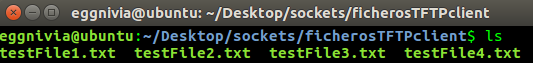
\includegraphics[scale=0.6]{images/client_before_1}
\caption{ficherosTFTPclient}
\end{figure}

Los archivos guardados en el servidor son los siguientes:

\begin{figure}[H]
\centering
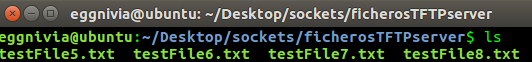
\includegraphics[scale=0.6]{images/server_before_1}
\caption{ficherosTFTPserver}
\end{figure}

La ejecución del programa será la siguiente:

\begin{figure}[H]
\centering
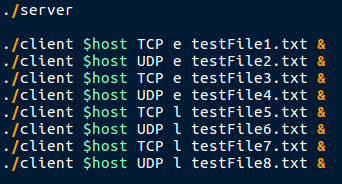
\includegraphics[scale=0.6]{images/script_prueba_1}
\caption{Script prueba 1}
\end{figure}

Tras la ejecución del programa se comprueba el log común para todos los clientes y el log del servidor. Se observa como las conexiones se han realizado satisfactioramente en puertos diferentes. En la Figura 5 vemos como aparecen las cuatro conexiones TCP que se han establecido durante esta primera prueba.

\begin{figure}[H]
\centering
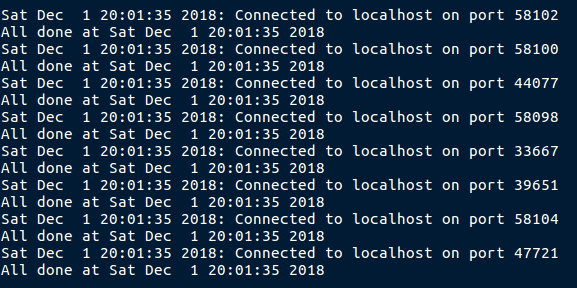
\includegraphics[scale=0.55]{images/log_cliente_prueba_1}
\caption{Log cliente prueba 1}
\end{figure}

\begin{figure}[H]
\centering
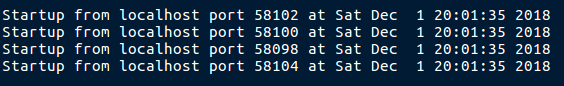
\includegraphics[scale=0.6]{images/log_server_prueba_1}
\caption{Log servidor prueba 1}
\end{figure}

Mirando los directorios, se comprueba como los archivos se han recibido de forma satisfactoria.

\begin{figure}[H]
\centering
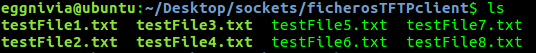
\includegraphics[scale=0.6]{images/client_after_1}
\caption{ficherosTFTPclient}
\end{figure}

\begin{figure}[H]
\centering
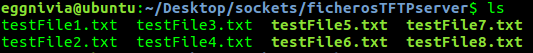
\includegraphics[scale=0.6]{images/server_after_1}
\caption{ficherosTFTPserver}
\end{figure}

La siguiente prueba, con el objetivo de forzar un error, se ha realizado inmediatamente después de la anterior. Como existen los mismos ficheros en ambos directorios, se deberá errores de existencia de archivos, tanto para los clientes como para el servidor.

\begin{figure}[H]
\centering
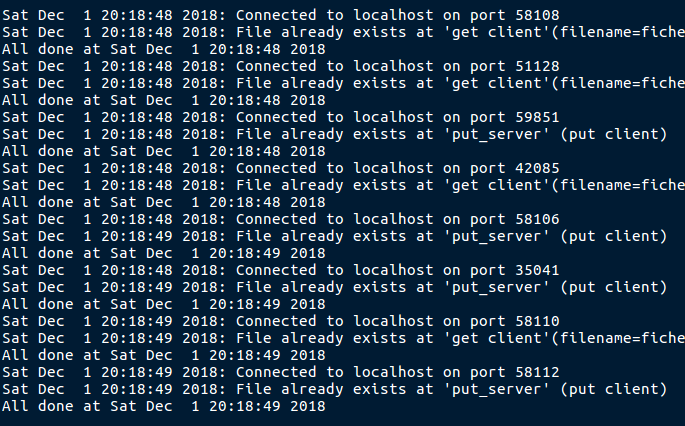
\includegraphics[scale=0.4]{images/log_cliente_prueba_2}
\caption{Log cliente prueba 2}
\end{figure}

En efecto, se observan dos tipos de errores en el log de los clientes: un tipo de error generado por los mismos clientes al intentar  hacer una operación de lectura (get) para un archivo que ya existe en su directorio, y otro tipo, siendo un mensaje de error enviado por el servidor, indicando que ya existe el archivo a enviar.

\begin{figure}[H]
\centering
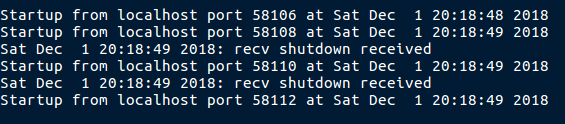
\includegraphics[scale=0.6]{images/log_server_prueba_2}
\caption{Log servidor prueba 2}
\end{figure}

En el log del servidor, se observan las conexiones TCP de modo análogo a la prueba anterior, pero además, los cierres de conexión (shutdown) de los clientes TCP de lectura, que abren una conexión en el socket solo para cerrarlas poco después al comprobar que ya existe el archivo que querian recibir.\\

La tercera prueba consistirá en lanzar el servidor en una máquina y un cliente en otra, en una subred diferente, para así comprobar que se envía de forma correcta un archivo a través de internet.\\

Para ello, se hace port-forwarding en el router a una máquina de la subred donde residirá el servidor. El cliente, por su parte, deberá indicar al ejecutarse que el host está en la IP pública del router del servidor, conectándose al puerto previamente abierto en el mismo.

% Your document ends here!
\end{document}